\title{Developing Inference Algorithms}

{{navbar}}

\subsubsection{Developing Inference Algorithms}

Edward uses class inheritance to provide a hierarchy of inference
methods. This enables fast experimentation on top of existing
algorithms, whether it be developing new black box algorithms or
new model-specific algorithms.

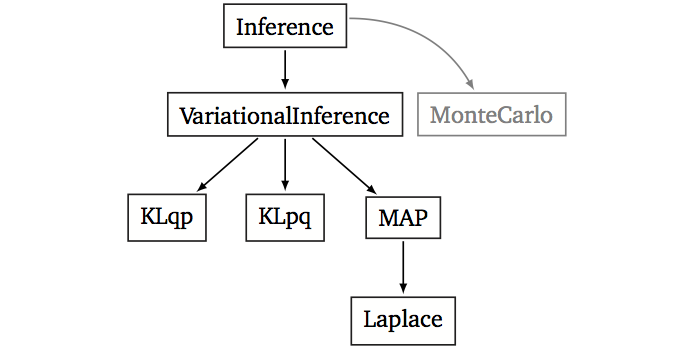
\includegraphics[width=700px]{/images/inference_structure.png}
{\small\textit{Dependency graph of inference methods.
Nodes are classes in Edward and arrows represent class inheritance.}}

There is a base class \texttt{Inference}, from which all inference
methods are derived from.

\begin{lstlisting}[language=Python]
class Inference(object):
  """Base class for Edward inference methods.
  """
  def __init__(self, latent_vars=None, data=None, model_wrapper=None):
    ...
\end{lstlisting}

It takes as input the set of latent variables to infer and a dataset. Optionally, if the user uses an external language to specify the model, it takes as input a model wrapper \texttt{model_wrapper}.

Note that \texttt{Inference} says nothing about the class of models that an
algorithm must work with. One can build inference algorithms which are
tailored to a restricted class of models available in Edward (such as
differentiable models or conditionally conjugate models), or even
tailor it to a single model. The algorithm can raise an error if the
model is outside this class.

We organize inference under two paradigms:
\texttt{VariationalInference} and \texttt{MonteCarlo} (or more plainly,
optimization and sampling). These inherit from \texttt{Inference} and each
have their own default methods.

\begin{lstlisting}[language=Python]
class MonteCarlo(Inference):
  """Base class for Monte Carlo inference methods.
  """
  def __init__(latent_vars, data=None, model_wrapper=None):
    super(MonteCarlo, self).__init__(latent_vars, data, model_wrapper)

  ...


class VariationalInference(Inference):
  """Base class for variational inference methods.
  """
  def __init__(self, latent_vars=None, data=None, model_wrapper=None):
    super(VariationalInference, self).__init__(latent_vars, data, model_wrapper)

  ...
\end{lstlisting}

For example, developing a new variational inference algorithm is as simple as
inheriting from \texttt{VariationalInference} or one of its derived
classes. \texttt{VariationalInference} implements many default methods such
as \texttt{initialize()} with options for an optimizer.

For examples of inference algorithms developed in Edward, see the inference
\href{/tutorials/}{tutorials}. It can also be useful to look at
the
\href{https://github.com/blei-lab/edward/tree/master/edward/inferences}
{source code}.
